    %%%% ijcai25.tex

\typeout{IJCAI--25 Instructions for Authors}

% These are the instructions for authors for IJCAI-25.

\documentclass{article}
\pdfpagewidth=8.5in
\pdfpageheight=11in

% The file ijcai25.sty is a copy from ijcai22.sty
% The file ijcai22.sty is NOT the same as previous years'
\usepackage{ijcai25}

% Use the postscript times font!
\usepackage{times}
\usepackage{soul}
\usepackage{url}
\usepackage[hidelinks]{hyperref}
\usepackage[utf8]{inputenc}
\usepackage[small]{caption}
\usepackage{graphicx}
\usepackage{amsmath}
\usepackage{amsthm}
\usepackage{booktabs}
\usepackage{algorithm}
\usepackage{algorithmic}
\usepackage[switch]{lineno}
\usepackage{subcaption}
\usepackage{color}
\def\oursys{KnowPath\xspace}
% Comment out this line in the camera-ready submission
% \linenumbers

\urlstyle{same}

% the following package is optional:
%\usepackage{latexsym}

% See https://www.overleaf.com/learn/latex/theorems_and_proofs
% for a nice explanation of how to define new theorems, but keep
% in mind that the amsthm package is already included in this
% template and that you must *not* alter the styling.
\newtheorem{example}{Example}
\newtheorem{theorem}{Theorem}

% Following comment is from ijcai97-submit.tex:
% The preparation of these files was supported by Schlumberger Palo Alto
% Research, AT\&T Bell Laboratories, and Morgan Kaufmann Publishers.
% Shirley Jowell, of Morgan Kaufmann Publishers, and Peter F.
% Patel-Schneider, of AT\&T Bell Laboratories collaborated on their
% preparation.

% These instructions can be modified and used in other conferences as long
% as credit to the authors and supporting agencies is retained, this notice
% is not changed, and further modification or reuse is not restricted.
% Neither Shirley Jowell nor Peter F. Patel-Schneider can be listed as
% contacts for providing assistance without their prior permission.

% To use for other conferences, change references to files and the
% conference appropriate and use other authors, contacts, publishers, and
% organizations.
% Also change the deadline and address for returning papers and the length and
% page charge instructions.
% Put where the files are available in the appropriate places.


% PDF Info Is REQUIRED.

% Please leave this \pdfinfo block untouched both for the submission and
% Camera Ready Copy. Do not include Title and Author information in the pdfinfo section
\pdfinfo{
/TemplateVersion (IJCAI.2025.0)
}

\title{KnowPath: Knowledge-enhanced Reasoning via LLM-generated Inference Paths over Knowledge Graphs}


% Single author syntax
\author{
    Qi Zhao\textsuperscript{1}, Hongyu Yang\textsuperscript{1}, Qi Song\textsuperscript{1}\thanks{Corresponding author}, Xinwei Yao\textsuperscript{2}, Xiangyang Li\textsuperscript{1}
    \affiliations
    \textsuperscript{1}University of Science and Technology of China, Hefei, Anhui, China \\ 
        \textsuperscript{2}Zhejiang University of Technology, Hangzhou, Zhejiang, China \\ 
    % Affiliation
    \emails
    \{zq2021, hongyuyang\}@mail.ustc.edu.cn \\ 
        xwyao@zjut.edu.cn, \{qisong09, xiangyangli\}@ustc.edu.cn\\
    % email@example.com
}
% \author{\textbf{Qi Zhao}\textsuperscript{1}, \textbf{Qi Song}\textsuperscript{1}\thanks{Corresponding author}, \textbf{Tian Xie}\textsuperscript{1}, \textbf{Haiyue Zhang}\textsuperscript{2}, \textbf{Hongyu Yang}\textsuperscript{1}, \textbf{Xiangyang Li}\textsuperscript{1} \\
%         \textsuperscript{1}University of Science and Technology of China, Hefei, Anhui, China \\ 
%         \textsuperscript{2}Columbia University, New York, NY, USA \\ 
%         \{zq2021, xie\_tian, hongyuyang\}@mail.ustc.edu.cn \\ 
%         hz2995@columbia.edu, \{qisong09, xiangyangli\}@ustc.edu.cn\\ 
% }
% Multiple author syntax (remove the single-author syntax above and the \iffalse ... \fi here)
\iffalse
\author{
First Author$^1$
\and
Second Author$^2$\and
Third Author$^{2,3}$\And
Fourth Author$^4$\\
\affiliations
$^1$First Affiliation\\
$^2$Second Affiliation\\
$^3$Third Affiliation\\
$^4$Fourth Affiliation\\
\emails
\{first, second\}@example.com,
third@other.example.com,
fourth@example.com
}
\fi

\begin{document}

\maketitle
\begin{abstract}
Testing Autonomous Driving Systems (ADS) is crucial for ensuring their safety, reliability, and performance. Despite numerous testing methods available that can generate diverse and challenging scenarios to uncover potential vulnerabilities, these methods often treat ADS as a black-box, primarily focusing on identifying system failures like collisions or near-misses without pinpointing the specific modules responsible for these failures. Understanding the root causes of failures is essential for effective debugging and subsequent system repair. We observed that existing methods also fall short in generating diverse failures that adequately test the distinct modules of an ADS, such as perception, prediction, planning and control.

To bridge this gap, we introduce \tool, the first root-cause-aware testing method for ADS. Unlike previous approaches, \tool not only generates scenarios leading to collisions but also showing which specific module triggered the failure. This method targets specific modules, creating test scenarios that highlight the weaknesses of these given modules. Specifically, our approach involves designing module-specific oracles to ascertain module failures and employs a module-directed testing strategy that includes module-specific feedback, adaptive seed selection, and mutation. This strategy guides the generation of tests that effectively provoke module-specific failures. We evaluated \tool across four critical ADS modules and four testing scenarios. The results demonstrate that our method can effectively and efficiently generate scenarios where errors in targeted modules are responsible for ADS failures. It generates 216.7 expected scenarios in total, while the best-performing baseline detects only 79.0 scenarios. 
Our approach represents a significant innovation in ADS testing by focusing on identifying and rectifying module-specific errors within the system, moving beyond conventional black-box failure detection.
\end{abstract}

\keywords{Module-Specific Failure, Autonomous Driving System, Testing}
Stochastic systems have been used extensively in several areas including  verification~\cite{FKNP11}, learning theory~\cite{AJKS21}, epidemic processes~\cite{Lef81} to name a few. Several real-world systems however do not work with a centralised control. Therefore, modelling using stochastic systems with multiple agents makes for more faithful abstractions of such systems without a centralised control. Some examples of fields in which multi-agents stochastic modelling include cyber physical systems~\cite{SEC16}, distributed and probabilistic computer programs~\cite{dAHJ01}, probabilistic planning~\cite{TKI10}. In such cases, the problem of reasoning about multiple agents with several, often times orthogonal objectives, becomes important. % However, for situations that are modelled as graph games, Nash equilibria come with its own down-sides and therefore several notions of equilibria have emerged in turn-based games on graphs to circumvent the problems posed by the natural definitions of Nash equilibira, like subgame-perfect equilibira, Stackleberg-equilibria. 
For multi-agent systems modelled with stochasticity on the underlying arena, a fundamental question to ask is the existence or finding of an equilibrium.
The most popular equilibria in literature are Nash equilibria~\cite{Nas50}. However, those come with their own downsides. The computational complexity for studying Nash equilibria over multi-agent systems is prohibitively expensive, and even undecidable in the general case, where systems have $10$ or more players~\cite{UW11}. 
Further, even if Nash equilibria could be computed efficiently, they do not faithfully model the agents in real world settings
%as each agent might perceive risk differently. With randomness arising from both the strategies of other agents, as well as the underlying model of the system, this might mean that risk-averse or risk-loving agents might have an incentive to deviate since their perceived values of outcome is different from expected value of the game.
since they do not consider their tolerance or averseness to risk.

Let us consider a $1$-player game where a protagonist is proposed two options: (a) earning \$1; (b) playing a lottery in which, with probability $\frac{1}{40}$, she gets \$40, and with probability $\frac{39}{40}$, she does not earn anything.
Classically, rational strategies would be maximising the expected payoff. From this perspective, both options yield an expected payoff of \$1, making them equivalent.
This approach is particularly justified when the game represents a scenario that can be repeated many times: the law of large numbers ensures that, in the long run, the average payoff will converge to the expected payoff. However, when the game is played only once, the protagonist may prioritise immediate needs. If she urgently requires \$1, the guaranteed option (a) becomes preferable.

Conversely, if she is a risk-taker or finds herself in a situation where only the \$40 can make a significant difference, she may prefer the high-risk option (b).
Although this choice might appear irrational, it mirrors the behaviour of millions of people who participate everyday in games with a negative expected payoff, driven by the allure of a potentially life-changing win, and generating an annual turnover of USD 536 billions~\cite{GamblingNewspaper23} for the gambling industry.
That industry, on the other hand, operates on a large scale where expected payoff becomes the key metric. 
This contrast underscores the importance of alternative measures to expected payoff that account for each agent's risk tolerance.%, offering a more nuanced understanding of decision-making in uncertain scenarios.

%We thus have an example of a two-player interaction, with apparently zero-sum payoffs, but where both players express a preference for the same option, because the context gives them a different tolerance to risk: this paradox underscores the importance of alternative measures to expected payoff that account for an agent's risk tolerance, offering a more nuanced understanding of decision-making in uncertain scenarios.
% This contrast underscores the relevance of generalising the notion of Nash equilibria: in a multi-agent system, the agents may have diverging perception of which risks can be taken.
% It makes sense, then, to study \emph{risk-sensitive equilibria}, in which players do not necessarily maximise their expected payoff, but their perception of what their payoff will be according to different risk measures.\leon{I'm actually not satisfied with this, I will modify it and move it.}


% Classically, we consider that a rational strategy would consist in maximising the expected payoff: from that perspective, the two choices are equivalent.
% Such an approach is justified especially when the game models a situation that can be repeated a large number of times, in which case the law of large numbers guarantees that the average payoff converges to the expected payoff.
% But when the game models a situation that is played only once, the protagonist may consider that she really needs her euro, and that the possibility of earning 40\$ is too unlikely to be taken into account: she would then have a justifiable preference for the option (a).
% On the contrary, if she is more of a gambler, or if she finds herself in a desperate situation in which only earning those 40\$ could save her, she could go all out and express a strict preference for option (b)\footnote{Even though this case seems more irrational, it explain why millions of people play everyday games in which they know that their expected payoff is negative.
% On the other side, the companies with whom they interact repeat the experience often enough to consider expected payoff as the relevant measure --- generating a yearly turnover of 536 billions of US\$.}.
% Hence the relevance of alternatives to expected payoff, that take into account the tolerance of the agent to risk.

\subparagraph*{Risk Measures.}
A \emph{risk measure} captures the perception that a player has of what their payoff will be. In that sense, they generalise the notion of expected payoff.
Various risk measures exist in the literature, and have been used extensively in the field of economics and finance. 
Some of these risk measures include expected shortfall (ES), value at risk (VaR)~\cite{Aue18}, variance~\cite{Bra99}, entropic risk measure (ER)~\cite{FS02}. 

%However, since the introduction of the characteristic of risk measure called \emph{coherence}~\cite{ADJH99}, it was expected that a ``good'' a risk measure must be coherent. A risk measure is coherent if it is monotonic, homogeneous, translational-invariance, and sub-additive.
%This automatically weeds out several of the above risk measures listed above like  Value at Risk or variance as a risk measure. 
A lot of work has been done in considering these risk measures over MDPs which use variance (along with mean) as a risk-measure~\cite{FK89, PSB22,MT11}, ES~\cite{RRS15,KM18,Meg22} (also referred to as conditional value at risk (CVaR), average value at risk (AVaR), expected tail loss (ETL), and superquantile in literature) and ER~\cite{HM72,BR14,BCMP24}. % have also been studied. 
Studying the entropic risk measure in MDPs appears more practical compared to expected shortfall  or using variance-penalised risk-measures. This impracticability of ES and variance-penalised measure in particular is due to the intractable exponential memory~\cite{HK15} and time required to compute optimal strategies~\cite{PSB22}, even for the one agent system of Markov decision processes (MDPs). On the other hand, when the risk measure used is ER, players have optimal positional strategies in MDPs~\cite{How72}, which makes it a prime candidate for consideration in multi-agent settings.

\subparagraph*{Entropic Risk Measure.}
The entropic risk measure is computed by assigning to each agent a risk parameter, i.e., a value $\rho \in \Rb$.
%Based on this risk parameter $\rho$, this measure first computes the expectation of the exponential function of the random variable and then re-normalises this.  
The entropic risk measure of a random variable $X$ is then defined as
$\re_\rho[X] = -\frac{1}{\rho} \log_e \left( \Eb \left[ e^{-\rho X}\right] \right)$. 
%For computational reasons, instead of the Euler's constant $e$, we use different bases sometimes.
If the risk parameter $\rho$ is positive, then more weight will be given to the bad payoffs: the corresponding player can then be considered as risk-averse.
Conversely, players with a negative $\rho$ are more risk-loving.
When $\rho$ tends to $0$, the entropic risk measure converges to the classical expectation $\Eb[X]$.

The game depicted by Figure~\ref{fig:example_gamma} extends the lottery example we discussed earlier. 
Black vertices are stochastic, and the circle vertex is controlled by player $\Circle$.
A play can be seen as an infinite sequence of moves of a token along the edges of the graph, starting from $a$: from a stochastic vertex, it takes one of the outgoing edges with the probabilities indicated on those, and from a vertex controlled by the player, she chooses which edge it takes.
The payoff $40$, $0$, or $1$ is obtained when the terminal vertex $t_1$, $t_2$, or $t_3$ is reached, respectively.
If no terminal vertex is reached, then the payoff is $0$.
Taking the red edge corresponds to option (a): then, her risk entropy is always $1$, for every risk parameter $\rho$.
But if she chooses option (b), that is, if she takes the blue edge, her risk entropy is $\re_\rho[\mu_{\circ}] = -\frac{1}{\rho} \log \left( \Eb \left[ e^{-\rho \mu_{\circ}}\right] \right) = -\frac{1}{\rho} \log \left(  e^{-40\rho } + \frac{39}{40} \right)$.
Both cases are illustrated with red and blue curves in \cref{fig:example_plot}.
The curves cross at abscissa $\rho = 0$, where the entropic risk measure corresponds to the expectation. Note that other strategies are possible if \emph{randomisation} is allowed---the player could, for example, toss a coin and participate in the lottery if the outcome is heads. The perceived reward of randomising between outermost red and blue edges are illustrated in the intermediate cases with mixtures of red and blue in \cref{fig:example_plot}.

%For this example, we  replace Euler's constant $e$ with instead the constant $2$, which makes $\re_\rho[X] = -\frac{1}{\rho} \log_2 \left( \Eb \left[ 2^{-\rho X}\right] \right)$.

%Player $\Circle$ gets the payoff $11$ if she reaches the terminal vertex $t_1$, the payoff $1$ if she reaches $t_2$, the payoff $2$ if she reaches $t_3$, and the payoff $0$ if she reaches none of those terminal states (i.e., if she loops on the vertex $a$ forever).

%If the player's strategy is to choose the red edge, she gets payoff $1$ with probability $1$.
%Therefore, her risk measure is equal to $1$ for every risk parameter $\rho$.

%If her strategy is to choose the blue edge going to $c$, then she gets the payoff $11$ with probability $\frac{1}{10}$, and $1$ with probability $\frac{9}{10}$.
%Thus her risk entropy is
%$\re_\rho[\mu_{\circ}] = \frac{1}{\rho} \log_2\left(\frac{1}{3} 2^{-4\rho} + \frac{2}{3} 2^{-1\rho}\right)$.
 
\begin{figure}[h] 
			\centering
            \begin{subfigure}[t]{0.4\textwidth}
			\begin{tikzpicture}[->,>=latex,shorten >=1pt, initial text={}, scale=1, every node/.style={scale=1}]
				\node[initial left, stoch] (a) at (0, 0) {$a$};
				\node[state] (b) at (1.5, 0) {$b$};
                \node[stoch] (c) at (2.5, 1) {$c$};
                \node (t1) at (4, 2) {$t_1:~\stack{\circ}{40}$};
                \node (t2) at (4, 0) {$t_2:~\stack{\circ}{0}$};
                \node (t3) at (3, -1) {$t_3:~\stack{\circ}{1}$};
                \path (a) edge[loop above] node[above] {$\frac{1}{2}$} (a);
				\path (a) edge node[above] {$\frac{1}{2}$} (b);
                \path (b) edge[blue, thick] (c);
                \path (b) edge[red, thick] (t3);
				\path (c) edge node[above] {$\frac{1}{40}$} (t1);
				\path (c) edge node[below] {$\frac{39}{40}$} (t2);
			\end{tikzpicture}
			\caption{A stochastic MDP}
			\label{fig:example_gamma}
            \end{subfigure}
            \begin{subfigure}[t]{0.55\textwidth}
			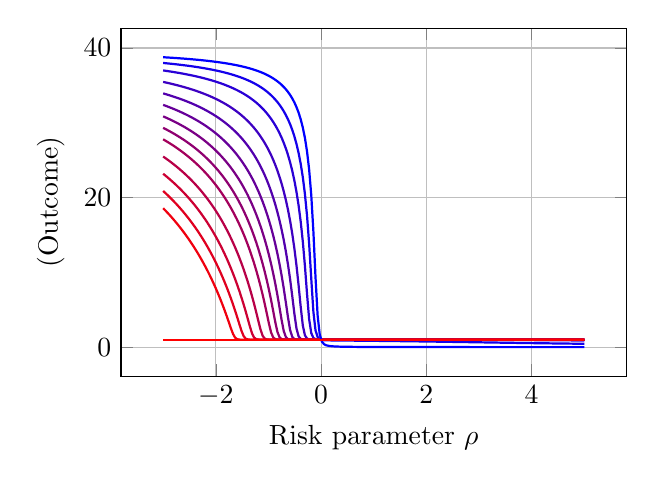
\begin{tikzpicture}
              \begin{axis}[
                xlabel={Risk parameter $\rho$},
                ylabel={$\re(\text{Outcome})$},
                domain=-3:5,
                samples=200,
                    width=8cm,
                   height=6cm,
                grid=major,
                ]
                \addplot [
                  red!8!blue,
                  thick
                ]
                {-1/x * log2((9/10)*e^(-1*x) + (1/400) * e^(-40*x) + (39/400))/log2(e)};
                \addplot [
                  red!16!blue,
                  thick
                ]
                {-1/x * log2((199/200)*e^(-1*x) + (1/8000) * e^(-40*x) + (39/8000))/log2(e)};
                \addplot [
                  red!24!blue,
                  thick
                ]
                {-1/x * log2((19999/20000)*e^(-1*x) + (1/800000) * e^(-40*x) + (39/800000))/log2(e)};
                \addplot [
                  red!32!blue,
                  thick
                ]
                {-1/x * log2((1999999/2000000)*e^(-1*x) + (1/80000000) * e^(-40*x) + (39/80000000))/log2(e)};
                \addplot [
                  red!40!blue,
                  thick
                ]
                {-1/x * log2((199999999/200000000)*e^(-1*x) + (1/8000000000) * e^(-40*x) + (39/8000000000))/log2(e)};
                \addplot [
                  red!48!blue,
                  thick
                ]
                {-1/x * log2((19999999999/20000000000)*e^(-1*x) + (1/800000000000) * e^(-40*x) + (39/800000000000))/log2(e)};
                \addplot [
                  red!56!blue,
                  thick
                ]
                {-1/x * log2((1999999999999/2000000000000)*e^(-1*x) + (1/80000000000000) * e^(-40*x) + (39/80000000000000))/log2(e)};
                \addplot [
                  red!64!blue,
                  thick
                ]
                {-1/x * log2((199999999999999/200000000000000)*e^(-1*x) + (1/8000000000000000) * e^(-40*x) + (39/8000000000000000))/log2(e)};
                \addplot [
                  red!72!blue,
                  thick
                ]
                {-1/x * log2((199999999999999999/200000000000000000)*e^(-1*x) + (1/8000000000000000000) * e^(-40*x) + (39/8000000000000000000))/log2(e)};
                \addplot [
                  red!80!blue,
                  thick
                ]
                {-1/x * log2((199999999999999999999/200000000000000000000)*e^(-1*x) + (1/8000000000000000000000) * e^(-40*x) + (39/8000000000000000000000))/log2(e)};
                \addplot [
                  red!88!blue,
                  thick
                ]
                {-1/x * log2((199999999999999999999999/200000000000000000000000)*e^(-1*x) + (1/8000000000000000000000000) * e^(-40*x) + (39/8000000000000000000000000))/log2(e)};
                \addplot [
                  red!94!blue,
                  thick
                ]
                {-1/x * log2((199999999999999999999999999/200000000000000000000000000)*e^(-1*x) + (1/8000000000000000000000000000) * e^(-40*x) + (39/8000000000000000000000000000))/log2(e)};
                \addplot [
                  blue,
                  thick
                ]
                {-1/x * log2((1/40) * e^(-40*x) + (39/40))/log2(e)};
                \addplot [
                  red,
                  thick
                ]
                {+1};
              \end{axis}
            \end{tikzpicture}
			\caption{Each curve represents the perceived reward of a player choosing only blue strategy, only red, or  randomising between both strategies. The percieved payoff for a player with risk parameter $\rho \in (-3,5)$ for these strategies are represented.}
			\label{fig:example_plot}
            \end{subfigure}
        \caption{Entropic risk measure}\label{fig:example_re}
\end{figure}
%\end{example}
Unfortunately, even for two player zero-sum stochastic games with total-reward objectives (payoff is the sum of the rewards seen along the way), computing optimal strategies can only be done in $\PSPACE$, when the base $e$ is replaced by an algebraic number; and if $e$ is the base of the exponent, then it is decidable only subject to Shanuel's conjecture~\cite{BCMP24}. % and inputs where the risk is computed using ER. 
Solving the two-player zero-sum case is a specific case of finding equilibria in two-agent systems where the payoffs of the two agents are exactly the negation of each others and so are the risk parameters of each of the agents.
Therefore, reasoning about multi-agent systems with ER also has potential to be computationally intractable.%\leon{I'm not sure I understand this sentence}


% \subparagraph*{Equilibria}
% Our example involves only one player.
% However, one might model it with a second player: the company that sells the lottery ticket, and therefore that made the choice of making the game possible.
% Of course, in the real world, companies only enable such games when its expected payoff is positive, that is, when the player's expected payoff is negative; which does not prevent millions of players to participate in such lotteries everyday, generating an annual turnover of USD 536 billion~\cite{h2_gambling_2023}.
% This can be explained by the fact that players are ready to take an important risk there, because they play a small number of times, and their likely loss remains acceptable, while their possible earning would be huge: in other words, players are efficiently modelled by a negative risk parameter.
% On the other hand, the company repeats the game a very large number of times, which is why, from its perspective, the expected payoff is the relevant metric.
% %This contrast underscores the importance of alternative measures to expected payoff that account for an agent's risk tolerance, offering a more nuanced understanding of decision-making in uncertain scenarios.
% This contrast underscores the relevance of generalising the notion of Nash equilibria: in a multi-agent system, the agents may have diverging perception of which risks can be taken.
% It makes sense, then, to study \emph{risk-sensitive equilibria}, in which players do not necessarily maximise their expected payoff, but their perception of what their payoff will be according to different risk measures.\leon{I'm actually not satisfied with this, I will modify it and move it.}



\subparagraph*{Extreme Risk Measure.} We introduce a new risk measure called extreme risk measure (XR) to identify tractable risk parameters. %\leon{Do we actually use that notation?} 
% If they have to choose between two options: (a) one which always gives him an outcome of 1, and the other option (b) that gives him a positive probability $p$ of 100, but  probability $(1-p)$ of -1, he would always chose option (a), 
%
%Let us say in a stochastic system, one agent is tasked with a safety-critical objective and wishes to avoid any positive probability of getting a payoff below some threshold, say $0$.
Consider an agent who wishes to maximise the lowest payoff received with positive probability.
In our example, 
by choosing option (a) her only payoff is $\$1$, whereas by choosing option (b), the payoffs that she receives with positive probability are $\$40$ and $\$0$. 
This agent would choose the option (a) since, then, the lowest reward she gets is $\$1$, instead of $\$0$. This would be her choice regardless of the probabilities or if the lottery amount in option (b) is increased.
%Even when the probabilities are changed for option (b) or if the lottery amount is increased, she would still prefer option (a).
Such agents can be considered ``extreme pessimists'' because
their perceived payoff can be thought of as the minimum among all the possible payoffs.
%We define the perceived reward of an extreme pessimist as the infimum of the payoffs that they get with positive probability. Therefore, extreme pessimists aim to maximise the smallest payoff that they receive with positive probability, and might be willing to deviate to achieve this objective.  
Similarly, one can define ``extreme optimists''  whose perceived reward is the best payoff that can be obtained with positive probability.
In the above scenario, an extreme optimist posed with the same options would choose option (b), no matter how small the probability is of receiving that payoff.

Extreme pessimists can be used to model safety-critical agents, where any positive probability of low reward or failure is unacceptable.
On the other hand, extreme optimists model naturally the opponents of such agents.
In a multiplayer setting, they can be an accurate modelling of agents like hackers in a system, who are happy with a small probability of success, or agents that have the possibility to restart their interactions with the same system, so that as long as there is a non-zero probability of achieving a high reward, they are guaranteed to receive that high reward. %\theju{If at all we discuss motivation here is the space.}





%\begin{example}
% Consider the same example game as in \cref{fig:example_gamma}. Here, the reward that the player perceives in the MDP can perceive on using the red strategy is exactly $2$ since that is the only payoff the player can get with a positive probability.
% However, if using the blue strategy, the perceived reward depends on if the player is an optimist or a pessimist. If the players is a pessimist, then the perceived reward is $4$, and if instead the player is an extreme pessimist, then the perceived reward is $1$.
%\end{example}
% \thejaswini{Introduce with examples some systems that need to be designed where some agent needs sure reward, and agents that some agents are happy with non-zero probability of reward}

%We capture this concept of extreme optimism and pessimism by introducing a new risk measure of pessimistic expectation and optimistic expectation.
\subparagraph*{Our results.}
We consider the problem of finding equilibria in a multiplayer stochastic game, that is, a game in which the payoffs that the players receive depend on the \emph{terminal vertex} that is reached, and in which an infinite play is associated to the zero payoff vector.

Our contributions are four fold. 
Firstly, we consider the problem of finding equilibria where entropic risk measure is used to determine the perceived reward of each player.  Each player has their own risk-sensitivity parameter, and we wish to find an equilibrium where no player has the incentive to deviate and increase their risk measure. We show that, when the rewards are all non-negative, such an equilibrium always exists.
We conjecture that this remains true when rewards can be negative.
Although some equilibria exist, not all equilibria are made the same, with some equilibria being more desirable than the others. One might want to find an equilibrium that maximises the overall social welfare, or want to minimise it for certain agents. A reasonably general setting is providing an interval for the risk measure for each agent and to check if there is an equilibrium satisfying these constraints. We call this problem \emph{constrained existence problem of risk-sensitive equilibria} (RSEs). 
We show (in \cref{sec:ERM}) that this problem is undecidable when the risk parameters of the players are rational values, with undecidability results extending from the constrained existence problem for Nash equilibria in the work of Ummels and Wojtczak~\cite{UW11}. However, we find restrictions on strategies to recover decidability. % for risk-sensitive equilibria in the cases where the risk parameters are finite.
If we restrict the memory requirements of each player, then for (small) finite memory strategies, we can solve the problem by encoding it using the existential theory of reals with exponentiation, giving us decidability subject to Shanuel's conjecture, and $\PSPACE$ algorithms when the base of the exponents are encoded as small algebraic instances, reminiscent of the two-player zero-sum case by Baier et al.~\cite{BCMP24}. 
%(\cref{proposition:Undecidable}).

Secondly, since the general problem is undecidable, and even in restricted cases, we obtain complexities that are $\PSPACE$ or higher, we pivot to searching for a more tractable risk measure that can be used to find equilibria in multi-agent systems. We define extreme risk measure (XR) as a novel risk measure to consider in multi-agent stochastic systems. We show (in \cref{sec:XR}) that our new definition is robust, since it exactly captures the well-studied entropic risk measure when the risk parameters tend to $\pm \infty$.
%This result (\cref{thm:RE=PEorOE}) in turn ensures that our risk measure is a robust definition since it is the limit of a well-studied risk measure. 
We further show the existence of 
such equilibria for games with non-negative rewards. Moreover, there exists a stationary strategy profile that can be algorithmically constructed in polynomial time. We conjecture, again, that this remains true when negative rewards are involved.
One further advantage of XR as a risk measure is that it is indifferent to the exact probabilities of the underlying stochastic model, since it only deals with events that occur with a positive probability and, therefore, can also be used in systems where the underlying probabilities are unknown. 

Thirdly, we show that the constrained existence problem of RSEs is decidable and also $\NP$-complete when the perceived payoff is calculated using XR, where each agent is either an extreme optimist or pessimist. The $\NP$ membership is nontrivial and follows several steps. First, we show that if there is a strategy that satisfies the constraints, then there is a finite abstraction of this strategy. Later, we show that this finite abstraction of the strategy has a polynomial representation. 
With this polynomial representation of the strategy, we show that verifying whether a given polynomially represented strategy is a risk-sensitive equilibrium that satisfies the constraints can also be done in polynomial time. 
Finally, we show that if all players are extreme optimists, this problem is $\PTIME$-complete.%, and provide a polynomial time algorithm for the constrained existence problem.
%\thejaswini{We add to this list by introducing a new risk measure that captures the above situation of extreme optimism and pessimism.}
%\thejaswini{We argue that our definition is robust, since this exactly captures the ERisk measure when the parameters are set to $-\infty$ and $+\infty$}
% \thejaswini{When the parameters are anywhere that are not $\pm\infty$, we show that computing Equilibria where ERisk is the outcome is undecidable. }
% \thejaswini{Argue that however, computational costs of precisely computing RSE for such values for stochastic games are undecidable}
% \thejaswini{This makes our definition the only decidable fragment for finding equilibria with entropic risk as a measure decidable}
\section{Method}
\label{sec:method}

\subsection{Weaknesses of Previous Conditioning Methods}

The most popular form of latent image conditioning typically converts conditioning signals to images, before processing them with typical image processing models. While this approach is powerful, it exhibits limitations in handling complex image synthesis tasks, particularly when incorporating heterogeneous or sparse input conditions. Some approaches, such as \textit{LayoutDiffusion} \cite{zheng_layoutdiffusion_2024}, tackle this with custom attention modules that attend to bounding boxes with learned positional embeddings. However, these approaches neglect to include multiple modalities and the relationships between them, which overlooks nuanced interactions between conditioning signals i.e. disambiguating spatial ordering between overlapping boxes. 

% For example, interactions between conditions which may not explicitly exist in the discrete spatial image domain.

% These approaches force diverse modalities, like mixed spatial and categorical information directly into a unified image space, which overlooks nuanced interactions between conditioning signals. For example, interactions between conditions which may not explicitly exist in the discrete spatial image domain.

Previous conditional diffusion research that utilise graph data opt for complex multi-stage training procedures such as masked contrastive pre-training using graph triplets \cite{yang_diffusion-based_2022}. This is not only time-consuming, but also fails to exploit potential benefits of training an end-to-end system that integrates graph data directly into image processing. 
% Furthermore, other work has shown that the repeated conditioning diffusion models (i.e. time or text conditioning) is superior to simply providing   

We tackle these problems by representing images and their conditioning signals as a single graph, which is processed by a bespoke GNN architecture. This allows repeated interactions between conditioning signals and the image throughout the synthesis process, enabling more flexible and dynamic representations that account for both the current image features and interactions between conditioning signals. By maintaining separate pathways for distinct input types, our approach supports heterogeneous and sparse conditioning, leading to better generalisation, finer control, and more precise manipulation of generated images. This simple yet powerful method can be easily integrated into a wide range of existing vision models.

\begin{figure}
    \centering    \includegraphics[width=1\linewidth]{icml2023/hig_fig2.pdf}
\vspace{-20pt}
    \caption{(\textbf{a}) Overview of the proposed architecture. The HIG is encoded into a latent representation through a MP-GNN which is then used as a condition $c_f$ in a ControlNet. (\textbf{b}) Details of the MP-GNN module. Note: HMP is shorthand for heterogenous magnitude preserving operations applied across all nodes.}
    \label{fig:architecture}
\end{figure}

\subsection{Heterogeneous Image Graphs}

To improve on previous approaches we develop a new approach to condition images via the HIG representation. In this manner, we fully exploit variable-length and heterogeneous conditions to aid in image synthesis.

\textbf{Image Graphs.} When faced with the challenge of conditioning images with graphs we first convert images into representations amenable for graph processing. We reshape image features into image nodes pixel-wise in line with other works \cite{liu_cnn-enhanced_2021, han_vision_2022}. In practice, these nodes represent more than a single pixel, for example a latent image patch. This can be due to performing latent image diffusion \cite{rombach_high-resolution_2022, podell_sdxl_2023} where images are first pre-compressed to latent images, or due to prior processing by the image processing model. In contrast to other works \cite{tian_image_nodate, han_vision_2022, tarasiewicz_graph_2021}, we decide to leave image nodes unconnected; this loosely decouples image conditioning from processing. Image nodes are conditioned and later converted back into an image representation, allowing existing architectures to handle processing. Connecting image nodes in a locally dense fashion gains little benefit over highly optimised $3 \times 3$ convolutional operations. Formally, image nodes exist in a discrete space \( f : \mathbb{Z}^2 \to \mathbb{R}^C \). For an image of size \(M \times N\), we define \( f(i, j) \) where \( i, j \in \mathbb{Z} \) and \( 0 \leq i < M \), \( 0 \leq j < N \).

\textbf{Conditioning Graphs}. Conditioning graphs consist of nodes and edges, where each node has features defined as $ g : \mathcal{V} \to \mathbb{R}^F$, where $\mathcal{V}$ represents the set of nodes and $\mathbb{R}^F$ the feature space. Nodes may have spatial ties to the image domain, which we materialise via edges linking image and conditioning nodes. We use conditioning nodes to indicate semantics within the scene, for instance, a node may represent an object (e.g., a \textit{person}). Whereas we utilise different edge types to represent both spatial, abstract relationships and additional semantics. For instance, an edge between two object nodes may encode interactions or attributes (e.g., a person \textit{wearing} a {\textit{yellow}} hat). The graph structure reflects real-world data: often sparse and heterogeneous. We therefore construct graphs on a per task-basis to best leverage the available data and its dependencies.
Formally, each edge \( e \in \mathcal{E} \) connects two nodes \( (v_i, v_j) \in \mathcal{V} \times \mathcal{V} \) and represents a relationship between them. Edges represent any dependency, allowing for abstract relationships to be included.

% To continue the example, if spatial information for both the \textit{person} and the \textit{hat} is available, the graph would contain a node for each object and an edge connecting them, with the edge encoding the relationship \textit{wearing}. 


% \textbf{Conditioning Graphs.} In contrast, conditioning graphs are represented by sets of nodes and edges, with each node having associated features defined by a function $( g : \mathcal{V} \to \mathbb{R}^F$, where $\mathcal{V}$ represents the set of nodes and $\mathbb{R}^F$ the feature space. Although nodes \textit{may} have explicit spatial ties to the discrete image domain, we materialise these through edges between image and conditioning nodes. However, these relationships may be the product of spatial properties of conditioning nodes. As such, subsets of $\mathbb{R^F}$ may represent spatial coordinates \( (x, y) \in \mathbb{R}^2 \) that satisfy \( 0 \leq x < M \) and \( 0 \leq y < N \). Conditioning nodes are not restricted to pixel grid positions, nor the number of spatial dimensions e.g. nodes may represent 3D properties of the real world. Nodes and edges may represent properties independent of spatial dimensions. For example, nodes in the graph can represent concrete objects in the image (e.g., a \textit{person}), while edges between them may represent abstract interactions or attributes (e.g., a person \textit{wearing} a {\textit{yellow}} hat). The graph structure may be sparse, and heterogeneous (multiple types of nodes and edges). Conditioning graphs are constructed on a per-task basis to optimally leverage available data and its dependencies. Formally, each edge \( e \in \mathcal{E} \) connects two nodes \( (v_i, v_j) \in \mathcal{V} \times \mathcal{V} \) and represents a relationship between them. To continue the example, if spatial information for both the \textit{person} and the \textit{hat} is available, the graph would contain a node for each object and an edge connecting them, with the edge encoding the relationship \textit{wearing}. Edges can represent any dependency, allowing for abstract relationships to be included in the graph.

\textbf{Connecting Image and Conditioning Nodes.} With image and conditioning nodes defined, we are close to the complete HIG representation. To enable conditioning between the image and conditioning graphs, we must construct edges between the two. These connections are determined on a per-task basis, depending on the available data, with explicit choices described in Section 4. However, when spatial information is available i.e. segmentation masks or bounding boxes, it enables direct connections between the image graph and the conditioning graph. Specifically, edges are created between image nodes relevant to spatial conditionings (i.e. pixels within the bounding box) and conditioning nodes representing the corresponding semantic class (i.e. class label). This linkage facilitates information flow across the graphs, integrating pixel-level details with higher-level semantic representations. 

% Additionally, the flexibility of heterogeneous GNNs allows for connections from the image back to the graph with different sets of learned weights. This approach enables the image to influence the graph structure while leveraging the rich semantic details present in the image—such as color or object sub-class—throughout much of the diffusion training scheme, while still respecting the different types of information carried by the node types.

\subsection{Model Architecture}

To be compatible with the EDM2 U-Net architecture \footnote{\href{https://github.com/NVlabs/edm2}{https://github.com/NVlabs/edm2}}, we propose the addition of a magnitude-preserving \textit{Heterogenous Image Graph Neural Network} (HIGnn) as the conditioning network to be used in a ControlNet strategy.

\textbf{HIGnn.} The general architecture of the HIG conditioning block requires two primary capabilities: representation switching and HIG processing. To handle switching between image features and image nodes on the HIG we consider the update function $\mathcal{U}_{\text{i}\rightarrow\text{g}}$. This update functions reshapes image features $\mathbf{x_i} \in \mathbb{R}^{N \times C \times H \times W}$ into image nodes pixel wise $\mathbf{x_g} \in \mathbb{R}^{N\cdot H \cdot W \times C}$ and applies an optional projection to ensure correct dimensionality. For the current set of image pixels $\mathbf{x_i}$, we retrieve HIG image nodes $\mathbf{x_g}$ by
\begin{equation}
\mathbf{x_g} = \mathcal{U}_{\text{i}\rightarrow\text{g}}(\mathbf{x_i}) = \hat{W}R(\mathbf{x_i}),  
 \label{eq:HIG_update}
\end{equation}
where $R$ reshapes the image, and $\hat{W}$ is a learned projection with forced magnitude preservation from \cite{karras_analyzing_2024}. Refer to Appendix \ref{appendix:edm2_preliminaries} for greater detail into the mathematical preliminaries of \cite{karras_analyzing_2024}. We consider the reverse operation of converting from graph nodes to an image $\mathcal{U}_{\text{g}\rightarrow\text{i}}$ in a similiar fashion. 

Once we have the HIG updated with current image nodes we can process it with a GNN. We identify several areas where magnitudes can grow and address them each in turn. In practice many varieties of heterogenous message passing GNN could be used, we create our own magnitude preserving graph convolutional operator similiar to Hamilton et al. \cite{hamilton_inductive_2018} for its simplicity and stability. The basic approach propagates information through two branches, a pseudo `skip-connection' applied to the current node, and a learned pooling operation of the local neighbourhood, and we add the ability to include edge information in the neighbourhood pooling. If edge attributes $\mathbf{a}_i$ are present we integrate them via magnitude preserving concatenation to the pooling branch. Formally, the HIGConv operator applied per meta-path to get updated node embeddings $\mathbf{x}_i'$ is defined as:
% \begin{equation}
%     \mathbf{x}_i' = \psi\left(\hat{W}^{\Phi}_1 \mathbf{x}_i +^\text{mp} \hat{W}^{\Phi}_2 \cdot \frac{1}{\sqrt{|\mathcal{N}^{\Phi}|}} \sum_{j \in \mathcal{N}^{\Phi}(i)} [\mathbf{x}_j \|^\text{mp} \mathbf{a}_j] \right),
%     \label{eq:hignn_operator}
% \end{equation}
\begin{equation}
    \mathbf{x}_g' = \psi\left(\hat{W}^{\Phi}_1 \mathbf{x}_g 
    \underset{0 \text{ if } |\mathcal{N}^{\Phi}(i)| = 0}{\underbrace{+^\text{mp} \hat{W}^{\Phi}_2 \cdot \frac{1}{\sqrt{|\mathcal{N}^{\Phi}(i)|}} \sum_{j \in \mathcal{N}^{\Phi}(i)} [\mathbf{x}_j \|^\text{mp} \mathbf{a}_j]}}\right)    \label{eq:hignn_operator}
\end{equation}

% \[
%     \mathbf{x}_i' = \psi\left(\hat{W}^{\Phi}_1 \mathbf{x}_i +^\text{mp} 
%     \underset{+ 0 \text{ if } |\mathcal{N}^{\Phi}(i)| = 0}{\underbrace{\hat{W}^{\Phi}_2 \cdot \frac{1}{\sqrt{|\mathcal{N}^{\Phi}(i)|}} \sum_{j \in \mathcal{N}^{\Phi}(i)} [\mathbf{x}_j \|^\text{mp} \mathbf{a}_j]}}\right).
% \]

where we choose $\psi$ to be magnitude preserving SiLU operator, and $+^\text{mp}$ the magnitude preserving sum (See Appendix \ref{appendix:edm2_preliminaries}), and both meta-path weights $\hat{W}^{\Phi}_1$ and $\hat{W}^{\Phi}_2$ have forced magnitude. $\mathcal{N}$ indicates the local node neighbourhood and is defined by the connectivity of graph. In order to achieve magnitude preservation we first assume all neighbourhood features to be of unit length, we then summate them scale them by the square root of the neighbourhood size ($\sqrt{|\mathcal{N}^{\Phi}|}$), see Appendix \ref{appendix:sum_random} for details. It is important to address unconnected or `zero-degree' nodes, in this case we ignore the right hand side of the equation, and only take the residual path. Note that simply setting the  neighbourhood to zero unintentionally changes the feature magnitudes when mp-sum is applied, since it assumes both vectors to be of unit length. Finally to combine information across meta-paths, we use the same method and sum across paths before normalising by the inverse square root of the number of incoming meta-paths ($|\Phi_i| = |\{\Phi_k \mid x_i \in \Phi_k\}|$)

% To formulate a heterogeneous GNN with learned projections per meta-path ($\mathbf{\Phi} = \{\Phi_1 ... \Phi_n\}$), we must preserve magnitudes when combining meta-paths.

\begin{equation}
\Tilde{\mathbf{x}}_g = \frac{1}{\sqrt{|\Phi_g|}} \sum_{\Phi \in \Phi_g} \mathbf{x}'_g,
\label{eq:meta_path}
\end{equation}

We verify that this approach is guaranteed to maintain magnitudes under certain conditions of the underlying graph data. In particular, for graph-data of sufficient size this approach holds for graphs which do not have identical features attached to the same node since this breaks the independence assumption. 

% An interesting interpretation of this formulation with respect to image synthesis is to observe how different receptive fields change. The typical convolutional operator used in U-Net models define a local image receptive field $\mathcal{R}$, self-attention  defines a global image receptive field $\mathcal{A}$, and the HIGnn defines receptive fields over meta-path relationships $\mathcal{N}^{\Phi}$ for both the image and conditioning variables. We postulate this to an advantage over other conditioning methods as it allows instant communication between different conditioning signals and parts of the image whilst remaining computationally tractable.

\textbf{EDM2 ControlNet Integration.} To integrate conditioning into a generative model, we adopt a strategy similar to ControlNet \cite{zhang_adding_2023}, i.e. a frozen EDM2 pre-trained model, with a trainable copy the encoder integrated with the conditioning HIGnn. Refer to Figure \ref{fig:architecture} for an overview of our proposed architecture, we employ 4 HIG blocks for our base model. The EDM2 checkpoints are only available for class-conditional generation of the 1000 ImageNet classes, yet we find them easy to adapt to our natural image datasets.  To facilitate this we unfreeze the embedding network. To integrate features we adopt $1\times1$ convolutions with a learnable zero-gain in a similar fashion to the original ControlNet, but we note that traditional summation may damage feature magnitudes. We find that naively integrating is harmful to training. Instead, we apply magnitude preserving summation, which, in contrast to the original ControlNet paper, directly alters the primary network features. This yields poor generative quality at step 0, but proves to be quick to train and to be best in practice.

In the trainable encoder we integrate our proposed HIGnn after the initial convolution block. We opt to keep the dimension of the GNN matched to that of the generative model. Finally, to generate samples we opt for the non-stochastic EDM2 sampler, and use the recent advancements in auto-guidance \cite{karras_guiding_2024}, we use our control model as the primary network, and use the unconditional XS ImageNet checkpoint released with EDM2 as the guidance network \cite{karras_analyzing_2024, karras_guiding_2024}. 

% We do not use EMA
\section{Experimental Setup}\label{sec:exp}
\begin{table*}[ht]
\centering
\tabcolsep=0.35cm
\begin{tabular}{lcccc}
\toprule
\textbf{Method}              & \textbf{CWQ} & \textbf{WebQSP} & \textbf{Simple Questions} & \textbf{WebQuestions} \\ 
\midrule
\multicolumn{5}{c}{\textbf{LLM only}} \\
\midrule
IO prompt~\cite{ioprompt}                    & 37.6 $\pm$ 0.8         & 63.3 $\pm$ 1.2            & 20.0 $\pm$ 0.5              & 48.7 $\pm$ 1.4               \\ 
COT~\cite{cot}                          & 38.8 $\pm$ 1.5         & 62.2 $\pm$ 0.7            & 20.5 $\pm$ 0.4              & 49.1 $\pm$ 0.9               \\ 
RoG w/o planning~\cite{rog}             & 43.0 $\pm$ 0.9         & 66.9 $\pm$ 1.3            & -                 & -                  \\ 
SC~\cite{sc}                           & 45.4 $\pm$ 1.1         & 61.1 $\pm$ 0.5            & 18.9 $\pm$ 0.6              & 50.3 $\pm$ 1.2               \\ 
\midrule
\multicolumn{5}{c}{\textbf{Fine-Tuned KG Enhanced LLM}} \\ 
\midrule
UniKGQA~\cite{unikgqa}           & 51.2 $\pm$ 1.0         & 75.1 $\pm$ 0.8          & -        & -         \\
RE-KBQA~\cite{re-kbqa}  & 50.3 $\pm$ 1.2         & 74.6 $\pm$ 1.0            & -                 & -        \\
ChatKBQA~\cite{chatkbqa}                     & 76.5 $\pm$ 1.3         & 78.1 $\pm$ 1.1            & 85.8 $\pm$ 0.9              & 55.1 $\pm$ 0.6                  \\ 
RoG~\cite{rog}     & 64.5 $\pm$ 0.7         & 85.7 $\pm$ 1.4            & 73.3 $\pm$ 0.8    & 56.3 $\pm$ 1.0               \\ 
\midrule
\multicolumn{5}{c}{\textbf{Prompting KG Enhanced LLM with GPT3.5}} \\ 
\midrule
StructGPT~\cite{structgpt}      & 54.3 $\pm$ 1.0         & 72.6 $\pm$ 1.2        & 50.2 $\pm$ 0.5      & 51.3 $\pm$ 0.9          \\
ToG~\cite{tog}                          & 57.1 $\pm$ 1.5         & 76.2 $\pm$ 0.8            & 53.6 $\pm$ 1.0              & 54.5 $\pm$ 0.7               \\ 
PoG~\cite{pog}                          & 63.2 $\pm$ 1.0         & 82.0 $\pm$ 0.9            & 58.3 $\pm$ 0.6              & 57.8 $\pm$ 1.2               \\ 
\textbf{KnowPath (Ours)}                   & \textbf{67.9 $\pm$ 0.6} & \textbf{84.1 $\pm$ 1.3}   & \textbf{61.5 $\pm$ 0.8}     & \textbf{60.0 $\pm$ 1.0}      \\
\midrule
\multicolumn{5}{c}{\textbf{Prompting KG Enhanced LLM with DeepSeek-V3}} \\ 
\midrule
ToG~\cite{tog}           & 60.9 $\pm$ 0.7     & 82.6 $\pm$ 1.0         & 59.7 $\pm$ 0.9      & 57.9 $\pm$ 0.8                  \\ 
PoG~\cite{pog}              & 68.3 $\pm$ 1.1        & 85.3 $\pm$ 0.9         & 63.9 $\pm$ 0.5       & 61.2 $\pm$ 1.3           \\ 
\textbf{KnowPath (Ours)}     & \textbf{73.5 $\pm$ 0.9}     & \textbf{89.0 $\pm$ 0.8}        & \textbf{65.3 $\pm$ 1.0}       & \textbf{64.0 $\pm$ 0.7}       \\ 
\bottomrule
\end{tabular}

\caption{Hits@1 scores (\%) of different models on four datasets under various knowledge-enhanced methods. We use GPT-3.5 Turbo and DeepSeek-V3 as the primary backbones. Bold text indicates the results achieved by our method.}
\label{tab:comparison}
\end{table*}

\subsection{Baselines}


We chose corresponding advanced baselines for comparison based on the three main paradigms of existing knowledge-based question answering.
1) The First is the LLM-only, including the standard prompt (IO prompt\cite{ioprompt}), the chain of thought prompt (CoT\cite{cot}), the self-consistency (SC\cite{sc}), and the RoG without planning (ROG w/o planning\cite{rog}).
2) The second is the KG-enhanced fine-tuned LLMs, which include ChatKBQA\cite{chatkbqa}, RoG\cite{rog}, UniKGQA\cite{unikgqa}, and RE-KBQA\cite{re-kbqa}.
3) The third is the KG-enhanced prompt-based LLMs, including Think on graph (ToG\cite{tog}), Plan on graph (PoG\cite{pog}), and StructGPT\cite{structgpt}. 
Unlike the second, this scheme no longer requires fine-tuning and has become a widely researched mode today.


\subsection{Datasets and Metrics}
\textbf{Datasets.}
We adopt four knowledge-based question answering datasets: the single-hop Simple Questions~\cite{simpleqa}, the complex multi-hop CWQ~\cite{cwq} and WebQSP~\cite{webqsp}, and the open-domain WebQuestions~\cite{webquestion}.

\noindent\textbf{Metrics.}
Following previous research ~\cite{pog}, we apply exact match accuracy (Hits@1) for evaluation.


\subsection{Experiment Details}
Following previous research ~\cite{pog}, to control the overall costs, the maximum subgraph exploration depth $D_{amx}$ is set to 3. Since the FreeBase~\cite{freebase} supports all the aforementioned datasets, we apply it as the base graph for subgraph exploration, and We apply GPT-3.5-turbo-1106 and DeepSeek-V3 as the base models.
All experiments are deployed on four NVIDIA A800-40G GPUs.
\section{Result}

% 主要实验结果
\subsection{Main results}

We conducted comprehensive experiments on four widely used knowledge-based question answering datasets. The experimental results are presented in Table \ref{tab:comparison}, and four key findings are outlined as follows:


\textbf{KnowPath performs the best.}
Our KnowPath outperforms all the Prompting-driven KG-Enhanced.
For instance, on the multi-hop CWQ, regardless of the base model used, KnowPath achieves a maximum improvement of about 13\% in Hits@1.
In addition, KnowPath outperforms the LLM-only with a clear margin and surpasses the majority of Fine-Tuned KG-Enhanced LLM methods.
On the most challenging open-domain question answering dataset WebQuestions, KnowPath achieves the best performance compared to strong baselines from other paradigms (e.g., PoG 61.2\% vs Ours 64.0\%). This demonstrates KnowPath's ability to enhance the factuality of LLMs in open-domain question answering, which is an intriguing phenomenon worth further exploration.


\textbf{KnowPath excels at complex multi-hop tasks.}
On both CWQ and WebQSP, KnowPath outperforms the latest strong baseline PoG, achieving an average improvement of approximately 5\% and 2.9\%, respectively.
On the WebQSP, DeepSeek-v3 with KnowPath not only outperforms all Prompting-based KG-Enhanced LLMs but also surpasses the strongest baseline ROG among Fine-Tuned KG-Enhanced LLMs (85.7\% vs 89\%). 
On the more challenging multi-hop CWQ, the improvement of KnowPath over the PoG is significantly greater than the improvement on the simpler single-hop SimpleQuestions (5.2\% vs 1.4\%).
These collectively indicate that KnowPath is sensitive to deep reasoning.


\textbf{Knowledge enhancement greatly aids factual question answering.}
When question answering is based solely on LLMs, the performance is poor across multiple tasks. For example, COT achieves only about 20.5\% Hits@1 on SimpleQuestions.
This is caused by the hallucinations inherent in LLMs.
Whatever method is applied to introduce the KGs, they significantly outperform LLM-only. 
The maximum improvements across the four tasks are 35.9\%, 27.9\%, 46.4\%, and 15.3\%. 
% with the least improvements being 22.5\%, 17.2\%, 41\%, and 9.7\%, respectively.
These further emphasize the importance of introducing knowledge graphs for generating correct answers.



\textbf{The stronger the base, the higer the performance.}
As DeepSeek-V3 is better than GPT-3.5, even though both are prompting-based knowledge-enhanced, their performance on all tasks shows a significant difference after incorporating our KnowPath.
Replacing GPT-3.5 with DeepSeek-V3, KnowPath achieved a maximum improvement from 67.9\% to 73.5\% on CWQ, and on Simple Questions, it improved by at least 3.8\%.
These findings indicate that the improvement in model performance directly drives the enhancement of its performance in knowledge-based question-answering.


\textbf{KnowPath is a more flexible plugin.}
Compared to fine-tuned knowledge-enhanced LLMs, our KnowPath does not require fine-tuning of the LLM, yet it outperforms most of the fine-tuned methods.
In addition, on the CWQ dataset, KnowPath with DeepSeek-V3 achieves performance that is very close to the strongest baseline, ChatKBQA, which requires fine-tuning for knowledge enhancement. On the WebQSP dataset, it outperforms ChatKBQA by about 11\% (78.1\% vs 89.0\%).
Overall, the resource consumption of KnowPath is significantly lower than that of Fine-Tuned KG-Enhanced LLMs.
This is because KnowPath improves performance by optimizing inference paths and enhancing knowledge integration, making it a more flexible and plug-and-play framework.


% 消融实验表格
\begin{table}[t]
\centering
\resizebox{\columnwidth}{!}{  % 将表格宽度调整为单栏宽度
\begin{tabular}{lcccc}
\toprule
\textbf{Method} & \textbf{CWQ} & \textbf{WebQSP} & \textbf{SimpleQA} & \textbf{WebQ} \\
\midrule
KnowPath & 73.5 & 89.0 & 65.3 & 64.0 \\
-w/o IPG & 67.3 & 84.5 & 63.1 & 61.0 \\
-w/o SE & 64.7 & 83.1 & 60.4 & 60.7 \\
Base & 39.2 & 66.7 & 23.0 & 53.7 \\
\bottomrule
\end{tabular}
}
\caption{Ablation experiment results on four knowledge-based question answering tasks. IPG stands for Inference Paths Generation module, while SE stands for Subgraph Exploration module.}
\label{table:ablation}
\end{table}
\begin{table}[t]
\centering
\resizebox{\columnwidth}{!}{  % 将表格宽度调整为单栏宽度
\begin{tabular}{lcccc}
\toprule
\textbf{Method} & \textbf{LLM Call} & \textbf{Total Token} & \textbf{Input Token}\\
\midrule
ToG & 22.6 & 9669.4 & 8182.9  \\
PoG & 16.3 & 8156.2 & 7803.0 \\
KnowPath & \textbf{9.9} & \textbf{2742.4} & \textbf{2368.9} \\
\bottomrule
\end{tabular}
}
\caption{Cost-effectiveness analysis on the CWQ dataset between our KnowPath and the strongly prompt-driven knowledge-enhanced benchmarks (ToG and PoG). The Total Token includes two parts: the total number of tokens from multiple input prompts and the total number of tokens from the intermediate results returned by the LLM. The Input Token represents only the total number of tokens from the multiple input prompts. The LLM Call refer to the total number of accesses to the LLM agent.}
\label{table:tokens}
\end{table}
% 消融实验分析
\begin{figure}[h]
  \centering
  \includegraphics[width=0.94\linewidth]{figure/Ablation.pdf}
  \caption{Comparison of KnowPath, its individual components, and strong baseline methods (ToG and PoG) on the performance across four commonly used knowledge-based question answering datasets.}
  \label{fig:ablation}
\end{figure}
\subsection{Ablation Study}
We validate the effectiveness of each component of KnowPath and quantify their contributions to performance.
Its results are presented in Table \ref{table:ablation}, and visualized in Figure \ref{fig:ablation}.
\begin{figure*}[h]
  \centering
  \includegraphics[width=0.24\linewidth]{figure/CWQ_efficiency.pdf}
  % \hspace{0.01\linewidth}
  \includegraphics[width=0.24\linewidth]{figure/WebQSP_efficiency.pdf}
  \hspace{0.01\linewidth}
  \includegraphics[width=0.24\linewidth]{figure/SimpleQA_efficiency.pdf}
  % \hspace{0.01\linewidth}
  \includegraphics[width=0.24\linewidth]{figure/WebQ_efficiency.pdf}
  \caption{Visualization of the cost-effectiveness analysis on four public knowledge-based question-answering datasets.}
  \label{fig:efficiency-analysis}
\end{figure*}
\begin{figure}[t]
  \centering
  \begin{subfigure}{0.49\linewidth}
    \includegraphics[width=\linewidth]{figure/Temperature.pdf}
    \caption{Exploration temperature}
      \label{fig:tempreture}
  \end{subfigure}
  \begin{subfigure}{0.49\linewidth}
    \includegraphics[width=\linewidth]{figure/Triples.pdf}
    \caption{The count of triples}

    \label{fig:triple}
  \end{subfigure}
  % \hspace{0.01\linewidth}
  \caption{Analysis of key parameters.}
  \label{fig:Parameter}
\end{figure}

\begin{figure*}[t]
  \centering
    \includegraphics[width=0.98\linewidth]{figure/case1.pdf}
  % \hspace{0.01\linewidth}
  \caption{The case study on the multi-hop CWQ and open-domain WebQuestions dataset. To provide a clear and vivid comparison with the strong baselines (ToG and PoG), we visualized the execution process of KnowPath}
  \label{fig:case}
\end{figure*}


%每个模块均有贡献
\textbf{Each component contributes to the overall remarkable performance.}
After removing each module, their performance on different datasets will decline. However, compared to the base model, the addition of these modules still significantly improves the overall performance.


\textbf{It is necessary to focus on the powerful internal knowledge of LLMs.}
Eliminating the Subgraph Exploration and relying solely on the internal knowledge mining of LLMs to generate reasoning paths and provide answers proves to be highly effective. 
It has shown significant improvement across all four datasets, with an average performance enhancement of approximately 21.6\%. The most notable improvement was observed on SimpleQA, where performance leaped from 23\% to 60.4\%.
This indicates that even without the incorporation of external knowledge graphs, the performance of the model in generating factual responses can be enhanced to a certain extent through internal mining methods.
However, without the guidance of internal knowledge reasoning paths, KnowPath has seen some performance decline across all tasks, especially in complex multi-hop CWQ and WebQSP.


\textbf{The most critical credible directed Subgraph Exploration is deep-sensitive.}
Removing the subgraph exploration leads to a significant decline in Knowpath across all tasks, averaging a drop of approximately 5.7\%. This performance dip is particularly pronounced in complex multi-hop tasks. For instance, on the CWQ, Knowpath without subgraph exploration experiences a nearly 9\% decrease.






\subsection{Cost-effectiveness Analysis}

To explore the cost-effectiveness of KnowPath while maintaining high accuracy, we conducted a cost-benefit analysis. In this experiment, we tracked the primary sources of cost, including the LLM Call, Input Token, and Total Token usage. The results are presented in the Table \ref{table:tokens}, and are visualized in Figure \ref{fig:efficiency-analysis}.
Our key findings are described as follows:


\textbf{The number of accesses to the LLM agent was significantly reduced.} Specifically, the LLM calls for TOG and POG was 2.28x and 1.64x of that in our KnowPath, respectively.
This exceptionally low cost can be attributed to the fact that the Subgraph Exploration does not limit the scale of the path search, and this can be broken down into three key reasons. First, in each round of subgraph exploration, only one relation exploration and one entity exploration are conducted. Second, the Evaluation-based answering only accesses the LLM once after each round of subgraph exploration to judge whether the current subgraph can answer the question. If it cannot, the next round is performed. Third, if the largest explored subgraph still cannot answer the question, KnowPath will rely on the Inference Paths Generation.



\textbf{The number of tokens used is saved by several times.}
Whether in Total Token or Input Tokens, KnowPath saves approximately 4.0x compared to TOG and POG. 
This is mainly since all the prompts used in KnowPath are based on the carefully designed zero-shot approach, rather than the in-context learning used by the previous, which require providing large context to ensure the factuality of the answers.
We explored the reasons behind this difference.
First, previous methods rely on more contextual information for in-context learning to ensure the correctness of the output.
Secondly, KnowPath fully leverages the powerful internal relevant knowledge and uses it as the input signal for the agent.
This not only provides more contextual reference but also significantly improves the accuracy and efficiency of relation and entity exploration in subgraph exploration, ensuring that the generated subgraph is highly relevant while enabling the most effective reasoning toward potential answers.



% 参数分析
\subsection{Parameter analysis}





% 在这个部分,我们分析了影响KnowPath性能的重要参数,探讨了以下问题:
% 子图探索时的温度系数有何影响?
% 在子图探索时,温度系数的变化会影响模型生成答案的发散程度。较低的温度系数会影响KnowPath的性能,因为模型生成的保守答案知识较少,而大模型在探索和选择实体与关系时需要依赖一定的自身知识。较高的温度系数也会损害KnowPath的性能,因为发散的答案可能偏离给定的候选集合。
% 大量实验表明0.4是最佳温度,正与其他现有工作一样
We analyze the key parameters that affect the performance of KnowPath on the WebQSP, and discuss the following issues:

\textbf{What is the impact of the temperature in Subgraph Exploration?}
We explore the optimal temperature from 0.2 to 1, and the relation between it and Hits@1 is shown in Figure \ref{fig:tempreture}.
During subgraph exploration, variations in the temperature affect the divergence of the model's generated answers. A lower temperature negatively impacts KnowPath's performance, as the model generates overly conservative answers with insufficient knowledge, while the LLM relies on its internal knowledge when exploring and selecting entities and relationships. A higher temperature also harms KnowPath, as the divergent answers may deviate from the given candidates.
Extensive experiments show that 0.4 is the optimal temperature, consistent with other existing works~\cite{pog}.


\textbf{How is the count of knowledge triples determined in Inference Paths Generation?}
We explored it with a step size of 15, and the relationship between the count of knowledge triples and Hits@1 is shown in Figure \ref{fig:tempreture}.
When the count is 0, KnowPath's performance is poor due to the lack of internal knowledge exploration. When the count is too large, such as 45, its performance is also suboptimal, as excessive exploration introduces irrelevant knowledge as interference. Extensive experiments show that 15 is the optimal.

\subsection{Case Study}



To provide a clear and vivid comparison with the strong baselines, we visualized the execution process of KnowPath, as shown in Figure \ref{fig:case}. 
In the CWQ, ToG and PoG can only extract context from the question, failing to gather enough accurate knowledge for a correct answer, thus producing the incorrect answer "Taiping Jing." In contrast, KnowPath uncovers large model reasoning paths that provide additional, sufficient information. This enables key nodes, such as "Taoism," to be identified during subgraph exploration, ultimately leading to the correct answer, "Zhuang Zhou."
In the WebQuestions, ToG is unable to answer the question due to insufficient information. 
Although PoG provides a reasoning chain, the knowledge derived from the reasoning process is inaccurate, and the final answer still relies on the reasoning of the large model, resulting in the incorrect answer "Blackburn Rovers."
In contrast, guided by Inference, KnowPath accurately identified the relationship "time.event.instance\_of\_recurring\_event" and, through reasoning with the node "2002-03-Football League Cup," ultimately arrived at the correct result node "Liverpool F.C."
Overall, KnowPath not only provides answers but also generates directed subgraphs, which serve as the foundation for trustworthy reasoning and significantly enhance the interpretability of the results.



% \noindent {\textbf{Neural Fields.}} 
% 3d shape (\cite{chen2019learning}, \cite{park2019deepsdf}, \cite{mescheder2019occupancy})
% 3D scene reconstruction (NeRF\cite{mildenhall2021nerf}, ; \cite{niemeyer2021giraffe}),

% Neural Fields (NeFs) map coordinates to signals, providing a compact and flexible continuous data representation~\citep{sitzmann2020implicit, tancik2020fourier}. They are widely used for 3D object and scene modeling~\citep{chen2019learning, park2019deepsdf, mescheder2019occupancy, genova2020local, niemeyer2021giraffe}. NeRF~\citep{mildenhall2021nerf} learns neural radiance fields for view synthesis, mapping spatial coordinates to colors and densities via differentiable volumetric rendering. Extensions include Mip-NeRF~\citep{barron2021mip} for multiscale representations, TensoRF~\citep{chen2022tensorf} for low-rank tensor factorization, and NeuRBF~\citep{chen2023neurbf} for radial basis function aggregation. Unlike these methods, which rely on pre-defined structured information, we infer geometric bases to encode spatial structure.



%RBF-based works (\cite{ramasinghe2021learning}, \cite{ramasinghe2022beyond}, NeuRBF~\cite{chen2023neurbf}, 


\noindent {\textbf{Neural Fields (NeFs) and Generalization.}} Neural Fields (NeFs) map coordinates to signals, providing a compact and flexible continuous data representation~\citep{sitzmann2020implicit, tancik2020fourier}. They are widely used for 3D object and scene modeling~\citep{chen2019learning, park2019deepsdf, mescheder2019occupancy, genova2020local, niemeyer2021giraffe}. However, how to generalize to new scenes without retraining remains a problem. 
Many previous methods attempt to use meta-learning to achieve NeF generalization. Specifically, gradient-based meta-learning algorithms such as Model-Agnostic Meta Learning (MAML)~\citep{finn2017model} and Reptile~\citep{nichol2018first} have been used to adapt NeFs to unseen data samples in a few gradient steps~\citep{lee2021meta, sitzmann2020metasdf, tancik2021learned}. Another line of work uses HyperNet~\citep{Ha2016HyperNetworks} to predict modulation vectors for each data instance, scaling and shifting the activations in all layers of the shared MLP~\citep{mehta2021modulated, dupont2022data, dupont2022coin++}. Some methods use HyperNet to predict the weight matrix of NeF functions~\citep{dupont2021generative, zhang20233dshape2vecset}. Transformers~\citep{vaswani2017attention} have also been used as hypernetworks to predict column vectors in the weight matrix of MLP layers~\citep{chen2022transformers, dupont2022coin++}. In addition, \cite{reizenstein2021common,wang2022attention} use transformers specifically for NeRF. Such methods are deterministic and do not consider the uncertainty of a scene when only partially observed. Other approaches model NeRF from a probabilistic perspective~\citep{kosiorek2021nerf, hoffman2023probnerf, dupont2021generative, moreno2023laser,erkocc2023hyperdiffusion}. For instance, NeRF-VAE~\citep{kosiorek2021nerf} learns a distribution over radiance fields using latent scene representations based on VAE~\citep{kingma2013auto} with amortized inference. Normalizing flow~\citep{winkler2019learning} has also been used with variational inference to quantify uncertainty in NeRF representations~\citep{shen2022conditional, wei2023fg}. However, these methods do not consider potential structural information, such as the geometric characteristics of signals, which our approach explicitly models.



\noindent {\textbf{Neural Processes.}} Neural Processes (NPs)~\citep{garnelo2018neural} is a meta-learning framework that characterizes distributions over functions, enabling probabilistic inference, rapid adaptation to novel observations, and the capability to estimate uncertainties. This framework is divided into two classes of research. The first one concentrates on the marginal distribution of latent variables~\citep{garnelo2018neural}, whereas the second targets the conditional distributions of functions given a set of observations~\citep{garnelo2018conditional, gordon2019convolutional}. Typically, MLP is employed in Neural Processes methods. To improve this, Attentive Neural Processes (ANP)~\citep{kim2019attentive} integrate the attention mechanism to improve the representation of individual context points. Similarly, Transformer Neural Processes (TNP)~\citep{nguyen2022transformer} view each context point as a token and utilize transformer architecture to effectively approximate functions.
Additionally, the Versatile Neural Process (VNP)~\citep{guo2023versatile} employs attentive neural processes for neural field generalization but does not consider the information misalignment between the 2D context set and the 3D target points. The hierarchical structure in VNP is more sequential than global-to-local. Conversely, PONP~\citep{gu2023generalizable} is agnostic to neural-field specifics and concentrates on the neural process perspective. In this work, we consider a hierarchical neural process to model the structure information of the scene. 



\section{Conclusion}
This paper explores two open-ended questions: 1) How to utilize multimodal interleaved documents for CLIP training. 2) How to effectively leverage both realistic and synthetic texts to enhance CLIP performance. To this end, we first establish a Real-World Data Extraction pipeline to extract high-quality images and texts. Then we design a hierarchical retrieval method to efficiently associate each image with multiple semantically relevant texts. To further enhance fine-grained visual information, we propose an image semantic augmented generation module for synthetic text production. Furthermore, we employ a semantic balance sampling strategy to improve dataset diversity, enabling better learning of long-tail concepts. Based on these innovations, we present \textit{RealSyn}, a dataset driven by both real and synthetic texts with three sizes: 15M, 30M, and 100M. We compare our dataset with other widely used datasets of equivalent scale for CLIP training. Models pre-trained on RealSyn consistently achieve state-of-the-art performance across various downstream tasks. Furthermore, extensive experiments confirm that \textit{RealSyn} significantly enhances contrastive vision-language representation learning and demonstrates robust scalability. We hope our work provides insights into vision-language representation learning.

%% The file named.bst is a bibliography style file for BibTeX 0.99c
\bibliographystyle{named}
\bibliography{ijcai25}

\end{document}

